\chapter*{Introduction}
\phantomsection
\addcontentsline{toc}{chapter}{Introduction}

\section{Urychlovač SPS a slow extrakce}
\subsection{Úvod do urychlovačů částic}
Urychlovač částic je zařízení, které, pomocí elektromagnetických polí, pohání nabité částice. Takové částice se pak mohou pohybovat rychlostí, která je blízká rychlosti světla. Urychlovače se využívají ve zdravotnictví, průmyslu a výzkumu. Ve zdravotnictví slouží zejména v~onkologii k~cílenému ozařování nádorové tkáně. Ve vědecké sféře se pak v rámci experimentů z oblasti částicové fyziky tyto urychlené částice nechávají narážet do sebe nebo do pevného terče, ať už za účelem zkoumání nových částic, antihmoty, či zkoumání vlastností hmoty při vysokých energiích.

Existují dva hlavní typy urychlovačů:
\begin{enumerate}
	\item \textbf{Lineární urychlovač (Linac)} -- Částice se pohybují po přímé dráze skrz sérii rezonančních dutin. Vysokofrekvenční elektrické pole je postupně urychluje, zatímco magnetické pole slouží pouze k udržení úzkého profilu paprsku. Výhodou je absence energetických ztrát způsobených změnou směru letu což je významné
	zejména u~lehkých částic, jako jsou elektrony.
	\item \textbf{Kruhový urychlovač} -- Částice obíhají v~uzavřené vakuové trubici. Silné dipólové elektromagnety zakřivují jejich dráhu, takže částice mohou stejným urychlovacím úsekem s elektrickým polem projít mnohokrát. To umožňuje dosáhnout extrémních energií na menším prostoru.
\end{enumerate}





\subsection{Princip synchrotronu}
Synchrotrony jsou kruhové urychlovače, které urychlují částice v uzavřené křivce. Mohou tedy dosáhnout větší energie urychlených svazků. Části synchrotronu fungují následovně:

\subsubsection{RF dutiny}
Pro zrychlení částic je potřeba elektrické pole. Aby však částice obíhala po uzavřené kruhové dráze, nelze použít statické elektrické pole, protože by částice po jedné periodě se ocitla na místě se stejným potenciálem a celková práce by byla nulová. Je tedy třeba použít střídavého elektrického pole. Pole kmitá frekvencí:
\begin{equation}
	f_\text{RF} = h\,f_\text{rev}
\end{equation}
\vspace{0.5em}
\noindent kde je: \\
\begin{tabular}{l l l}
	$f_\text{RF}$ & frekvence kmitů elektrického pole v dutinách & $[\text{Hz}]$ \\
	$f_\text{rev}$ & oběžná frekvence částice & $[\text{Hz}]$ \\
	$h$ & harmonické číslo () & $[-]$ \\
\end{tabular}

Harmonické číslo je bezrozměrné celé číslo, které říká, kolikrát pole v dutině zakmitá během jednoho oběhu částice. Zároveň udává, kolik stabilních oblastí je rozmístěno po obvodu, svazek je tedy rozdělen do shluků.

%IDEÁLNĚ SEM OBRÁZEK RF DUTINY


\subsubsection{Dipóly}
Dipóly jsou elektromagnety s dvěma magnetickými póly. Jejich působením se ohýbá dráha svazků do uzavřeného kruhu. S rostoucí energií urychlovaných částic musí růst magnetická indukčnost. \cite{Tecker2020} 

\subsubsection{Kvadrupóly a betatronové kmity}
Částice ve svazku se polohově nepatrně liší, bez vnějšího působení by se tedy vychýlily a narazily do stěny vakuové trubice. K takzvané fokusaci svazku se používají kvadrupólové magnety. Kvadrupólové magnety na svazek působí podobně jako optické čočky \cite{cern_how_accelerator_works}. Kvadrupól se nechází u urychlovačů ve formě čtyř magnetů. Pole kvadrupólu je na ose nulové a roste lineárně s výchylkou částice, takže na ni působí silou úměrnou výchylce, podobně jako
pružina \cite{Holzer2018}. Kvadrupól však vždy fokusuje pouze v~jedné rovině a ve druhé svazek rozostřuje. Fokusace v~obou rovinách se
proto dosahuje střídáním fokusujících a defokusujících
kvadrupólů~\cite{Holzer2018}. Prstenec SPS je tvořen šesti
sextanty, z~nichž každý obsahuje 18 takových
buněk~\cite[kap.~IV.A]{Etisken2023}.

\begin{figure}[htbp]
	\centering
	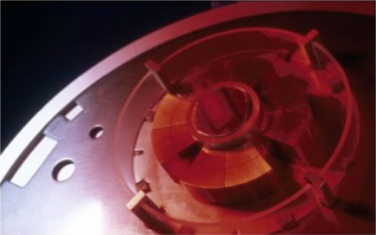
\includegraphics[width=0.8\textwidth]{pict/quadrupole_holzer2018.png}
	\caption{Superconducting quadrupole magnet in the LHC storage ring \cite[ch. 2.2]{Holzer2018}} 
	\label{fig:quadrupole_holzer2018}
\end{figure}

Vratná síla kvadrupólů způsobuje, že částice kolem ideální dráhy příčně
kmitají. Tyto kmity se nazývají betatronové a počet betatronových kmitů
během jednoho oběhu se nazývá tune~\cite[kap.~3]{Holzer2018}. V~SPS je
nominální horizontální tune $\nu_x = 26{,}66$ a vertikální
$\nu_y = 26{,}58$~\cite{Velotti}. Tune závisí na síle kvadrupólů, a lze ho
proto měnit nastavením jejich proudu. Této vlastnosti se využívá při
pomalé extrakci~\cite{Velotti} (viz kap.~\ref{sec:pomala_extrakce}). Když je hodnota tune blízko racionálního čísla, hrozí rezonance.

%DOPLNIT, DODĚLAT!!!
\subsubsection{Sextupóly}
Sextupóly pracují na podobném principu jako kvadrupóly, jsou to ale nelineární magnety. Působící síla na částici zde roste se čtvercem vzdálenosti. Sextupóly korigují chromaticitu a při pomalé extrakci budí rezonanci.\ref{sec:pomala_extrakce} Chromaticiotu se myslí pokles účinosti při vyšší hybnosti částice.\cite[ch. 4.2]{Holzer2018}


\subsection{Komplex urychlovačů CERN}
V rámci mezinárodní organizace CERN je provozováno vícero lineárních a kruhových urychlovačů. V rámci výzkumných experimentů je potřeba zapojit celou kaskádu urychlovačů, kde každý urychlovač urychlí protony na postupně větší a větší energii. Konec této kaskády tvoří Large Hadron Collider (LHC), kde energie částic může dosahovat až $6{,}8\,\text{TeV}$.~\cite{cern_accelerator_complex} 

Mezi nejznámější urychlovače se řadí Proton synchrotron s obvodem $628\,\text{m}$ \cite{gml_prednaska}, Super Proton Synchrotron s obvodem $6{,}9\,\text{km}$ \cite[kap.~IV.A]{Etisken2023} a Large Hadron Collider s obvodem $27\,\text{km}$ \cite{cern_LHC}

Celý proces začíná ionizací vodíku, při níž vznikají záporné vodíkové ionty
H$^-$. Lineární urychlovač Linac4 svazek těchto částic urychlí na $160\,\text{MeV}$. Při injekci do Proton Synchrotron Boosteru (PSB) jsou z~iontů odstraněny oba elektrony,
takže dále pokračují čisté protony. PSB urychlí protony na $2\,\text{GeV}$ a injektuje je do Proton Synchrotronu (PS), ze kterého už protony, urychlené na $25\,\text{GeV}$, následně putují do Super Proton Synchrotronu (SPS), kde dosahují energie až $450\,\text{GeV}$

Částice se urychlují pro různé experimety, které vyžadují určité parametry pro částice. Proto ne vždy je potřeba urychlovat částice až na úroveň LHC, často tedy jsou částice, nebo svazky částic odváděny už dříve. podobněji je to znázorněno na obr.~\ref{fig:cern_komplex_schema}.

\begin{figure}[htbp]
	\centering
	\includegraphics[width=1\textwidth]{pict/cern_accelerator_complex.png}
	\caption{Schéma akcelerátorového komplexu CERN} 
	\label{fig:cern_komplex_schema}
\end{figure}

\subsection{Super Proton Synchrotron}
Super Proton Synchrotron je druhý největší kruhový urychlovač v CERN o obvodu 6911,5~m \cite[kap.~IV.A]{Etisken2023}. Protony v něm obíhají s energií až $450 \,\text{GeV}$ a frekvencí $f_{rev} = 43{,}38 \,\text{kHz}$ \cite{DAQ_Belohrad}.

SPS je posledním urychlovačem v řetězci injektorů LHC, ale jeho hlavními uživateli jsou experimenty s pevným terčem v oblasti North Area \cite{Velotti} viz. \ref{fig:cern_komplex_schema} (viz obr.~\ref{fig:cern_komplex_schema}). Pro LHC jsou
protony urychlovány na $450\,\text{GeV}$, pro experimenty v~North Area na
$400\,\text{GeV}$~\cite{Velotti}.

\subsection{Pomalá rezonanční extrakce}
\label{sec:pomala_extrakce}

Svazek lze z kruhového urychlovače vyvést dvěma způsoby. Při rychlé extrakci
vychýlí rychlý magnet celý svazek během jediného oběhu. Takto se
plní (injektuje) například LHC. Experimenty s pevným terčem však vyžadují, aby byly
protony na terč dodávány co nejrovnoměrněji, tedy s~co nejvyšším tzv.
\emph{duty factorem} (viz kap.~\ref{sec:spill}). To vede k~nutnosti pomalé
extrakce, při níž se svazek vyvádí postupně po dobu několika
sekund~\cite{Velotti}.

Pro pomalou extrakci se v~SPS využívá třetinová rezonance (\emph{third-integer	resonance}), kterou budí extrakční sextupólové magnety~\cite{Velotti}. Síla
sextupólu roste s~kvadrátem výchylky částice~\cite[kap.~4.2]{Holzer2018}, takže
při každém průletu částici mírně vychýlí. Horizontální tune svazku se nastaví
těsně vedle hodnoty $80/3$, nominálně na $\nu_x = 26{,}66$~\cite{Velotti}.
Částice se pak v~sextupólech objevuje po každých třech obězích přibližně ve
stejné fázi svého betatronového kmitu, jejich působení se proto nevyruší, ale
sčítá, a amplituda kmitů roste.

% 3) KDO uteče a KAM (tvůj aktivní ¶2 + počet protonů z ř. 82–83)
Protože síla sextupólů roste s~výchylkou, rezonance ovlivňuje především
částice s~velkou amplitudou kmitů. Ve fázovém prostoru, tedy v~rovině tvořené
polohou a úhlem částice, tak vznikne stabilní oblast trojúhelníkového tvaru
ohraničená tzv. separatrix. Částice uvnitř této oblasti zůstávají na stabilních
trajektoriích. Částicím vně oblasti amplituda s~každými třemi oběhy roste, až
dosáhnou elektrostatického septa ZS, které je odkloní do extrakčního kanálu
a dále do přenosové linky TT20~\cite{Velotti}. Tímto způsobem lze vyvést až
$4\cdot10^{13}$ protonů za jeden spill~\cite{Velotti}.

% (volitelně) obrázek fázového prostoru u septa
% \begin{figure}[htbp]
	%   \centering
	%   \includegraphics[width=0.6\textwidth]{pict/velotti_fig5.png}
	%   \caption{Horizontální fázový prostor na vstupu elektrostatického septa ZS
		%            při pomalé extrakci. Převzato z~\cite[obr.~5]{Velotti},
		%            licence CC BY 3.0.}
	%   \label{fig:velotti_faze}
	% \end{figure}

% 4) PROČ to trvá sekundy (tvůj aktivní ¶3)
Velikost stabilní oblasti závisí na tom, jak blízko je tune rezonanci. Během
extrakce se síla kvadrupólů plynule mění, stabilní oblast se zmenšuje a částice
z~ní postupně vystupují~\cite{Velotti}. Díky chromaticitě $\xi_x = -1$ má
každá částice tune závislý na své hybnosti, a rezonance se tak dosahuje
postupně pro částice s~různou hybností~\cite{Velotti}. Svazek je tím vyváděn
rovnoměrně po dobu několika sekund.

% 5) CO se děje se shluky (z tvých ř. 69–74, zkráceno)
Aby měl svazek pro tento proces dostatečně široké rozložení hybností,
provádí se před extrakcí tzv. RF gymnastika, která rozložení hybností
rozšíří. Poté se napětí všech urychlovacích dutin nastaví na nulu a svazek
se rozplyne do spojitého proudu (debunchování). Tím se omezí modulace
vyvedeného svazku na frekvenci urychlovacího pole $200\,\text{MHz}$~\cite{Velotti}.

% 6) CO z toho plyne pro měření (tvůj aktivní ¶4)
Rychlost extrakce je tedy velmi citlivá na přesnou hodnotu tune. Jakékoli
zvlnění proudu v~kvadrupólových magnetech se proto projeví jako modulace
intenzity vyvedeného svazku (viz kap.~\ref{sec:spill}).

\subsection{Spill a frekvence zájmu}
\label{sec:spill}
%Spill je souvislý tok protonů vyvedených z~SPS během jedné pomalé
%extrakce. V~současném provozu trvá $4{,}8\,\text{s}$
%\cite{DAQ_Belohrad, TODO_Benitez2023}, což při oběžné frekvenci
%$43{,}38\,\text{kHz}$ odpovídá přibližně $2\cdot10^5$ oběhům. Specifikace
%počítá s~tím, že délka spillu nepřesáhne $10\,\text{s}$~\cite{DAQ_Belohrad}
%a pro budoucí experimenty může být kratší, až $1\,\text{s}$
%\cite{TODO_Benitez2023}.
%
%Ideální spill má konstantní okamžitou intenzitu. Jak vyplývá
%z~kap.~\ref{sec:pomala_extrakce}, rychlost extrakce je však velmi citlivá na
%přesnou hodnotu tune. Tune závisí na proudu v~kvadrupólových magnetech, takže
%i~malé zvlnění jejich napájecích zdrojů se projeví jako výrazná modulace
%intenzity spillu. Monitory spillu na SPS proto běžně zaznamenávají složky
%$50\,\text{Hz}$ a $100\,\text{Hz}$ pocházející z~napájení
%magnetů~\cite{TODO_Benitez2023}.
%
%Kvalitu spillu z~pohledu experimentů vyjadřuje duty factor
%\begin{equation}
%	F = \frac{\langle I \rangle^2}{\langle I^2 \rangle},
%	\label{eq:duty_factor}
%\end{equation}
%kde $I$ je okamžitá intenzita a $\langle\cdot\rangle$ značí střední hodnotu
%přes dobu spillu~\cite{TODO_experimenters_handbook}. Pro konstantní
%intenzitu je $F = 1$. Uvažujme spill se sinusovou modulací o~hloubce $m$,
%tedy $I(t) = I_0(1 + m\sin\omega t)$. Střední hodnota sinu je nulová
%a střední hodnota $\sin^2$ je $1/2$, odkud plyne
%\begin{equation}
%	F = \frac{I_0^2}{I_0^2\left(1 + m^2/2\right)} = \frac{1}{1 + m^2/2}.
%	\label{eq:duty_factor_sin}
%\end{equation}
%Každá spektrální složka spillu tedy duty factor snižuje. Znalost spektra
%spillu a jeho vývoje v~čase je proto pro optimalizaci extrakce
%klíčová~\cite{TODO_zadani}.
%
%Frekvence, které jsou ve spektru spillu z~provozního hlediska podstatné,
%shrnuje tab.~\ref{tab:frekvence_zajmu}.
%
%\begin{table}[htbp]
%	\centering
%	\caption{Frekvence zájmu ve spektru spillu
%		\cite{TODO_Benitez2023, DAQ_Belohrad, TODO_zadani}.}
%	\label{tab:frekvence_zajmu}
%	\begin{tabular}{lll}
%		\hline
%		Složka & Frekvence & Původ \\
%		\hline
%		Napájecí zdroje magnetů & 10\,Hz -- 10\,kHz & zvlnění proudu magnetů \\
%		Oběžná frekvence SPS & 43,38\,kHz, 86\,kHz & nerovnoměrné zaplnění prstence \\
%		Oběžná frekvence PS & 477\,kHz & časová struktura z~injektoru \\
%		RF systém SPS & 200\,MHz & nedokonalé debunchování \\
%		Harmonický RF systém & 800\,MHz & podélná stabilizace svazku \\
%		\hline
%	\end{tabular}
%\end{table}
%
%Složky od napájecích zdrojů vznikají mechanismem popsaným výše. Oběžná
%frekvence SPS a její druhá harmonická jsou důsledkem nerovnoměrného zaplnění
%prstence. Svazek tvoří dvě injekce o~délce $10{,}5\,\mu\text{s}$, za každou
%z~nich následuje mezera $1{,}05\,\mu\text{s}$ potřebná pro náběh kickeru
%odklápěče svazku~\cite{TODO_Benitez2023}. Součet
%$2\times(10{,}5 + 1{,}05)\,\mu\text{s} = 23{,}1\,\mu\text{s}$ odpovídá době
%oběhu, takže se v~intenzitě spillu opakují dvě mezery za oběh. Složka
%$477\,\text{kHz}$ je pozůstatkem časové struktury svazku z~injektoru
%PS~\cite{TODO_Benitez2023}. Obvod PS je jedenáctinou obvodu SPS, a proto
%$477\,\text{kHz} \approx 11 f_\text{rev}$.
%
%Složka $200\,\text{MHz}$ odpovídá frekvenci hlavního urychlovacího RF systému
%SPS~\cite{TODO_Hagmann2019}. Pokud debunchování svazku před extrakcí není
%dokonalé, zůstane ve spillu struktura s~periodou $5\,\text{ns}$ a ve spektru
%se objeví čára na této frekvenci~\cite{Velotti, DAQ_Belohrad}. SPS je dále
%vybaven RF systémem $800\,\text{MHz}$, který slouží k~podélné stabilizaci
%svazku, konkrétně k~Landauovu tlumení~\cite{TODO_Hagmann2019} a podélnému
%rozmítání svazku~\cite{TODO_Benitez2023}.
%
%Frekvence zájmu tedy pokrývají rozsah od jednotek hertzů po stovky
%megahertzů, tedy přes osm řádů. To klade značné nároky na měřicí systém,
%jehož princip popisuje následující kapitola.



\section{SPILL monitoring}

\subsection{monitory spill na SPS}
\subsection{Optické přechodové záření}
OTR - záblesk viditelného světla, který vznikne ve chvíli, kdy rychlá nabitá částice překročí hranici dvou prostředí s různými vlastnostmi. V praxi urychlovačů k tomu dochází typicky tehdy, když částice letící vakuem narazí na tenkou kovovou fólii.

Kde se toto záření bere:
Jak se letící proton blíží ke kovovému povrchu, jeho elektrické pole v kovu indukuje svůj zrcadlový obraz s opačným nábojem (zrcadlový náboj). Vzniká tak pomyslný elektrický dipól, jehož pole se s přibližováním extrémně rychle mění. V okamžiku, kdy proton fyzicky protne povrch fólie, se toto pole náhle zhroutí a přeskupí. Právě tato prudká skoková změna elektromagnetického pole se uvolní do prostoru jako vyzářená energie – a pokud částice letí dostatečně rychle, velká část této energie má vlnovou délku viditelného světla.

Průchod tenkou diagnostickou fólií svazek částic nevyhnutelně mírně rozptýlí a zhorší jeho kvalitu. Dějí se při tom tři hlavní fyzikální jevy:

Coulombův rozptyl (Rozostření svazku): Toto je nejvýraznější efekt. Kladně nabité částice (např. protony) prolétají kolem kladně nabitých jader atomů kovu ve fólii. Elektromagnetické síly je navzájem odpuzují, čímž se dráha letících protonů nepatrně odchýlí. Svazek se tak po průletu mírně „rozšíří“ do stran a ztratí svou původní dokonalou ostrost (zvětší se jeho divergence).

Ionizační ztráty (Zpomalení a zahřívání): Částice cestou narážejí do elektronů v atomech fólie a vyrážejí je ven. Předají jim tím zlomek své kinetické energie, čímž se prolétající částice nepatrně zpomalí a samotná fólie se zahřeje. Při extrémních energiích urychlovače SPS je ale tento úbytek rychlosti pro experimenty obvykle zanedbatelný.

Jaderné srážky (Ztráta částic): Zcela nepatrné procento částic se trefí čelně přímo do jádra atomu ve fólii. Tyto částice se srážkou roztříští, vytvoří sekundární záření a pro primární svazek jsou nenávratně ztraceny.

Právě proto se OTR fólie vyrábějí z co nejlehčích kovů (často titan nebo hliník) a jsou extrémně tenké, typicky jen jednotky mikrometrů. V případě vyváděného svazku (spill) projdou částice touto fólií pouze jednou na své konečné cestě k experimentu. Zmíněné drobné znehodnocení svazku je tak pro fyziky naprosto přijatelnou daní za to, že získají jeho přesný časový a prostorový profil.



\subsection{Fotonásobič a analogová úprava signálu}

\section{Aktuálně implementovaný měřicí řetězec}

\subsection{Hardwarová platforma}
\subsection{Formát dat a rozhraní ADC}
\subsection{režimy měření}
\subsection{Omezení součastného řešení}





\section{Základy číslicového zpracování signálu}
\subsection{vzorkování a kvantování}
\subsection{Diskrétní Fourierova transformace}
\subsection{Odhad spektra}
\subsection{Charakteristiky a metriky signálu}


\section{Softwarově definované radio}


\subsection{Princip digitální down-konverze}
\subsection{Numericky řízený oscilátor}
\subsection{Komplexní směšovač}


\subsection{Filtrace a decimace}
\subsubsection{FIR filtry}
FIR filtr je filtr, který má konečnou odezvu na jednotkový impulz, budu používat digitální, takže jde o počet koeficietů ($h[n] = b_0 + b_1z^{-1} + b_2z^{-2} +x\dots$), kde počet koeficientů, kterým se říká taps a jejich počet přímo odpovídá, kolik kroků bude trvat odezva na jenotkový impulz.

\begin{equation}
	h[n] = \sum_{i=0}^{N} b_i \cdot \delta[n-i] = 
	\left\{
	\begin{array}{ll}
		b_n & 0 \leq n \leq N \\
		0 & \mbox{otherwise}.
	\end{array}
	\right.
\end{equation}
\subsubsection{CIC filtry}
\subsubsection{decimace}


\subsection{FFT a streaming FFT}



\section{Implementace v FPGA}
\subsection{Aritmetika v pevné řádové čárce}
\subsection{Paralelní zpracování více vzorků za takt}
\subsection{Zdroje FPGA Arria V}




